\section{Experimentación y/o validación}

En base a los casos de uso implementados se realizó un análisis cualitativo y cuantitativo de cada ecosistema, con el objetivo de compararlos y ver las ventajas y desventajas de cada uno, teniendo en cuenta las siguientes categorías:

\begin{itemize}
    \item \textbf{Costos}: ¿Cuánto nos cuesta desplegar y mantener un servicio en cada ecosistema? ¿Un usuario final necesita efectuar algún costo monetario para el uso de la aplicación?
    \item \textbf{Experiencia de desarrollo}: ¿Qué tan fácil es desplegar en cada ecosistema? ¿Existen herramientas y documentación necesario que facilite el desarrollo?
    \item \textbf{Aplicabilidad al caso de uso}: ¿Qué tan viable es crear una aplicación comunitaria para cada uno de estos ecosistemas?
    \item \textbf{Performance}: ¿Cuánto tiempo tarda la creación y obtención de elementos en cada aplicación?
\end{itemize}

\subsection{Propiedades utilizadas para las métricas}

Para las distintas pruebas cuantitativas realizadas, se establecieron tamaños fijos según el tipo de contenido evaluado.

\subsubsection{Sitio Web Estático}

El sitio web estático se clasificó por el tamaño total del contenido alojado.

\begin{itemize}
    \item \textit{short}: sitio web de 5000 bytes de tamaño total.
    \item \textit{medium}: sitio web de 10000 bytes de tamaño total.
    \item \textit{large}: sitio web de 25000 bytes de tamaño total.
      "1KiB-50files"
  "25KiB-50files"
  "50KiB-1files"
  "50KiB-10files"
  "50KiB-25files"
  "50KiB-50files"

    
    \end{itemize}

\subsubsection{Repositorio de conocimiento}

Los artículos se separaron en tres clasificaciones, según su longitud en bytes:

\begin{itemize}
    \item \textit{short}: artículo de 5000 bytes.
    \item \textit{medium}: artículo de 10000 bytes.
    \item \textit{large}: artículo de 50000 bytes.
\end{itemize}

\subsubsection{Mensajero en tiempo real}

Para la medición del envío y recepción de mensajes, se consideró tres tipos de mensajes:

\begin{itemize}
    \item \textit{short}: mensaje de 1 palabra. ''\textit{Lorem}''
    \item \textit{medium}: mensaje de 10 palabras. ''\textit{Lorem ipsum dolor sit amet, consectetur adipiscing elit. Aliquam elementum.}''
    \item \textit{large}: mensaje de 30 palabras. ''\textit{Lorem ipsum dolor sit amet, consectetur adipiscing elit. Aliquam ex risus, porttitor sed lacus id, egestas lobortis purus. Curabitur consectetur metus ut est vehicula egestas. Class aptent taciti sociosqu ad.}''
\end{itemize}

El tamaño de las palabras elegidas representa el largo de los mensajes más comunes que suelen enviarse en un chat.

A partir de los datos obtenidos se calcularon el máximo (\textbf{Max}), mínimo (\textbf{Min}), la media (\textbf{Mean}), el desvío estándar (\textbf{Std}) y la mediana (\textbf{Median}) de cada muestra.
\subsection{IPFS}

Para realizar las métricas de IPFS, se utilizó el siguiente sistema:
\begin{itemize}
    \item \textbf{CPU:} Ryzen 5 1600
    \item \textbf{RAM:} 8GB
    \item \textbf{Almacenamiento:} SSD
\end{itemize}

\subsubsection{Costos}

Mientras que en una Blockchain convencional se delega el almacenamiento y cómputo en nodos dedicados a ese propósito a cambio de un monto monetaria, IPFS ejecuta todo de manera local. El costo de IPFS no es, entonces, monetario sino energético.

\subsubsection{Experiencia de desarrollo}

La experiencia de desarrollo dentro del ecosistema de IPFS resultó desafiante, principalmente debido a que se trata de una tecnología emergente y todavía poco adoptada en entornos de producción. Esto se tradujo en una falta de madurez en algunas herramientas clave y en una documentación a veces limitada o desactualizada.

En nuestro caso, se eligió trabajar con herramientas del ecosistema JavaScript, dado que OrbitDB está diseñado para este entorno y era necesario asegurar compatibilidad con navegadores web. No obstante, JavaScript no representa el entorno más maduro ni prioritario dentro de IPFS y libp2p, lo cual implicó enfrentar una serie de desafíos técnicos.

Durante el desarrollo, nos encontramos con múltiples situaciones en las que ciertas funcionalidades no se comportaban como se esperaba, o directamente no estaban implementadas. Esto nos llevó a participar activamente en los repositorios oficiales, creando distintos \textit{issues} y colaborando en la identificación y resolución de errores (ver Anexo \ref{anexo:issues-ipfs}).

Una de las principales limitaciones fue la falta de soporte para \textbf{WebRTC-Direct} en la implementación de LibP2P en JavaScript, una funcionalidad crítica para poder conectar nodos web con nodos independientes sin requerir servidores intermediarios. Esta característica se encontraba en pleno desarrollo durante el transcurso del proyecto, lo que implicó retrasos y momentos de incertidumbre respecto a la viabilidad técnica de la solución.

Afortunadamente, gracias al activo mantenimiento y la receptividad de los desarrolladores de las distintas herramientas involucradas, fue posible colaborar en la resolución de varios de estos problemas, seguir de cerca los avances en nuevas funcionalidades, y continuar con el desarrollo hasta alcanzar una infraestructura funcional y operativa.

\subsubsection{Aplicabilidad al caso de uso}

\subsubsection{Performance}

La performance en IPFS se ve afectada por algunas variables. Entre ellas se encuentran:

\begin{itemize}
    \item Uso de cache por parte de nodos de IPFS o gateways cuando se recupera un archivo.
    \item Cercanía al nodo correspondiente a la hora de publicar un CID en la Distributed Hash Table.
    \item Configuración y capacidades del nodo que tiene el contenido que se requiere.
    \item Cantidad de nodos alojando el contenido que se requiere.
\end{itemize}

 Se puede minimizar  el efecto de estas variables en la medida final sin distorsionar las métricas obtenidas. Más adelante se verán las maneras en las que se puede lidiar con estas variables.

\paragraph{Sitio Web Informativo}
La métrica que se decidió medir es la del \textbf{tiempo que tarda un nodo en desplegar un sitio web o contenido}. Para ello, se creó un clúster con un único nodo y un repositorio Git con contenido de distinta forma.

\subparagraph{Obtención de las métricas} En este caso, el proceso de despliegue se contiene dentro del contenedor \texttt{watcher}. Para medir el tiempo real que transcurre en cada paso del despliegue, se utilizó el comando de GNU \texttt{time} para cada paso, y el resultado es sumado para obtener el tiempo total que tardó desplegar el contenido.

\subparagraph{Variables consideradas} Las métricas obtenidas se lograron ajustando dos variables: el tamaño total del contenido, y la cantidad de archivos del mismo. Los archivos en sí fueron generados repitiendo un \texttt{UUID} hasta alcanzar el número de bytes deseados. Se utilizó este tipo de identificador para asegurar de que ningún archivo permanezca en alguna caché de la red o en la DHT, y a su vez no se repitan los CID entre archivos de la misma prueba.

\begin{figure}[H]
    \centering
    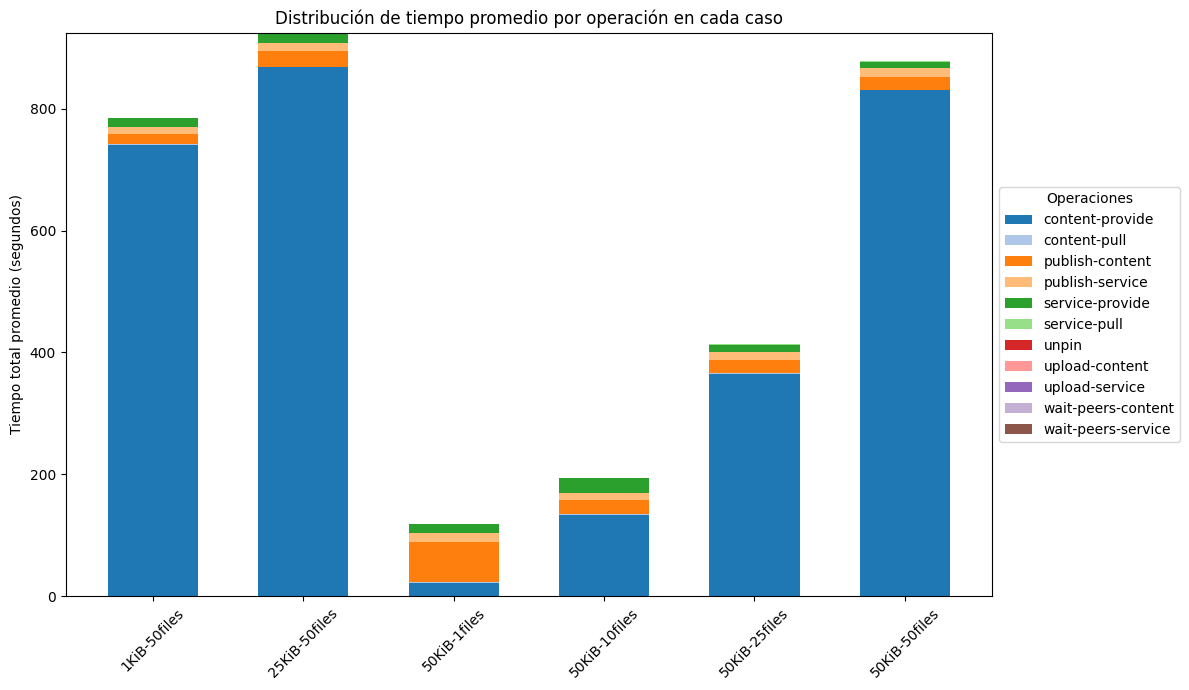
\includegraphics[width=1\linewidth]{img/metricas-ipfs/metricas-ipfs-caso1-1.png}
    \caption{Distribución del tiempo promedio para desplegar el contenido para cada caso}
    \label{fig:metricas-ipfs-caso1-1.png}
\end{figure}

De este gráfico podemos concluir que la operación más significante en términos de tiempo en el despliegue es la \textit{providing} del contenido. Esto es, la publicación de todos los CIDs en la DHT. Luego, le siguen el providing del \texttt{service.json}, y las operaciones para actualizar el valor al que apunta el nombre de IPNS, tanto del contenido como del \texttt{service.json}. Las demás operaciones se pueden despreciar.



\setlength\tabcolsep{10pt}
\begin{table}[!htbp]
    \centering
    \begin{tabular}{|c|c|c|c|c|c|}
    \hline
    & \textbf{Max} & \textbf{Mean} & \textbf{Min} & \textbf{Std} & \textbf{Median} \\
    \hline
    \textbf{1KiB-50files} & 23.65 s & 17.66 s & 7.70 s & 6.39 s & 21.71 s \\
    \hline
    \textbf{25KiB-50files} & 67.29 s & 25.92 s & 8.96 s & 15.24 s & 22.95 s \\
    \hline
    \textbf{50KiB-1files} & 78.75 s & 66.09 s & 61.48 s & 5.83 s & 62.93 s \\
    \hline
    \textbf{50KiB-10files} & 30.57 s & 12.93 s & 7.10 s & 7.42 s & 8.96 s \\
    \hline
    \textbf{50KiB-25files} & 23.79 s & 22.65 s & 21.94 s & 0.46 s & 22.57 s \\
    \hline
    \textbf{50KiB-50files} & 23.36 s & 20.95 s & 8.17 s & 4.27 s & 22.43 s \\
    \hline
    \end{tabular}
    \caption{Estadísticas para \texttt{publish-content}}
\end{table}

\setlength\tabcolsep{10pt}
\begin{table}[!htbp]
    \centering
    \begin{tabular}{|c|c|c|c|c|c|}
    \hline
    & \textbf{Max} & \textbf{Mean} & \textbf{Min} & \textbf{Std} & \textbf{Median} \\
    \hline
    \textbf{1KiB-50files} & 17.76 s & 10.30 s & 7.54 s & 3.39 s & 8.79 s \\
    \hline
    \textbf{25KiB-50files} & 23.03 s & 12.76 s & 7.31 s & 6.37 s & 8.74 s \\
    \hline
    \textbf{50KiB-1files} & 23.08 s & 15.37 s & 7.52 s & 6.71 s & 15.25 s \\
    \hline
    \textbf{50KiB-10files} & 23.31 s & 13.31 s & 7.34 s & 6.86 s & 8.44 s \\
    \hline
    \textbf{50KiB-25files} & 23.02 s & 12.17 s & 7.43 s & 5.80 s & 8.97 s \\
    \hline
    \textbf{50KiB-50files} & 22.85 s & 13.91 s & 7.28 s & 6.43 s & 11.32 s \\
    \hline
    \end{tabular}
    \caption{Estadísticas para \texttt{publish-service}}
\end{table}

\setlength\tabcolsep{10pt}
\begin{table}[!htbp]
    \centering
    \begin{tabular}{|c|c|c|c|c|c|}
    \hline
    & \textbf{Max} & \textbf{Mean} & \textbf{Min} & \textbf{Std} & \textbf{Median} \\
    \hline
    \textbf{1KiB-50files} & 851.26 s & 740.32 s & 682.64 s & 41.45 s & 734.15 s \\
    \hline
    \textbf{25KiB-50files} & 918.36 s & 868.11 s & 815.43 s & 26.57 s & 872.25 s \\
    \hline
    \textbf{50KiB-1files} & 42.09 s & 21.84 s & 10.79 s & 7.49 s & 20.14 s \\
    \hline
    \textbf{50KiB-10files} & 419.87 s & 372.47 s & 327.86 s & 25.09 s & 377.78 s \\
    \hline
    \textbf{50KiB-25files} & 412.30 s & 364.53 s & 306.15 s & 26.53 s & 366.01 s \\
    \hline
    \textbf{50KiB-50files} & 921.54 s & 830.06 s & 744.83 s & 41.12 s & 826.65 s \\
    \hline
    \end{tabular}
    \caption{Estadísticas para \texttt{content-provide}}
\end{table}

\setlength\tabcolsep{10pt}
\begin{table}[!htbp]
    \centering
    \begin{tabular}{|c|c|c|c|c|c|}
    \hline
    & \textbf{Max} & \textbf{Mean} & \textbf{Min} & \textbf{Std} & \textbf{Median} \\
    \hline
    \textbf{1KiB-50files} & 27.62 s & 14.83 s & 8.84 s & 6.12 s & 11.41 s \\
    \hline
    \textbf{25KiB-50files} & 34.34 s & 15.67 s & 10.99 s & 6.64 s & 11.66 s \\
    \hline
    \textbf{50KiB-1files} & 25.71 s & 13.63 s & 6.49 s & 5.26 s & 11.34 s \\
    \hline
    \textbf{50KiB-10files} & 20.88 s & 12.86 s & 10.84 s & 3.11 s & 11.30 s \\
    \hline
    \textbf{50KiB-25files} & 20.78 s & 12.42 s & 9.78 s & 3.47 s & 11.26 s \\
    \hline
    \textbf{50KiB-50files} & 20.27 s & 11.31 s & 6.82 s & 3.17 s & 10.97 s \\
    \hline
    \end{tabular}
    \caption{Estadísticas para \texttt{service-provide}}
\end{table}

Teniendo en cuenta esto, se puede observar cuál es la causa de la variación del tiempo de providing ajustando las dos variables mencionadas.

\begin{figure}[H]
    \centering
    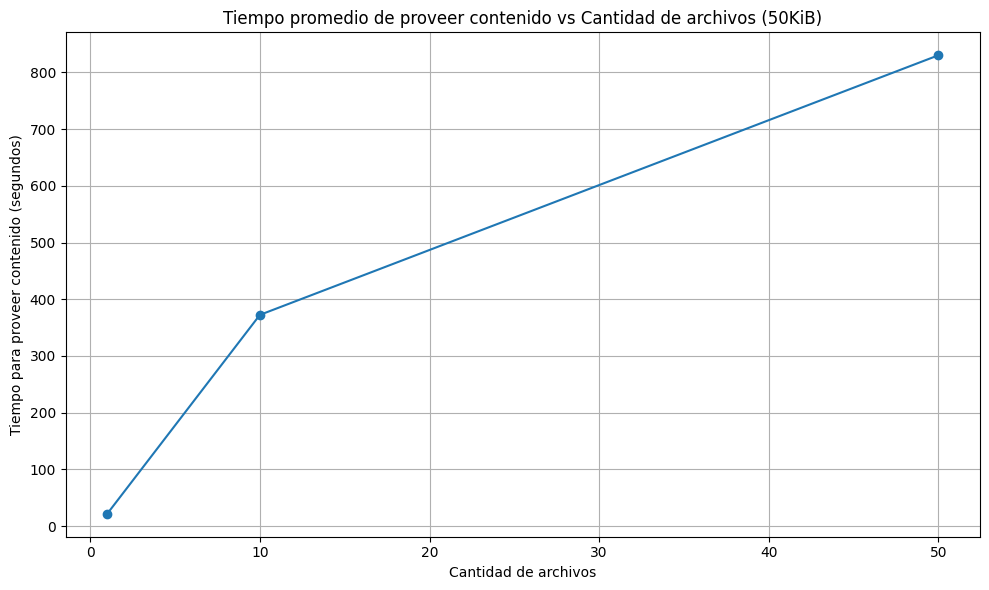
\includegraphics[width=1\linewidth]{img/metricas-ipfs/tiempo-por-cant-archivos.png}
    \caption{Tiempo promedio por cantidad de archivos}
    \label{fig:tiempo-por-cant-archivos.png}
\end{figure}

\begin{figure}[H]
    \centering
    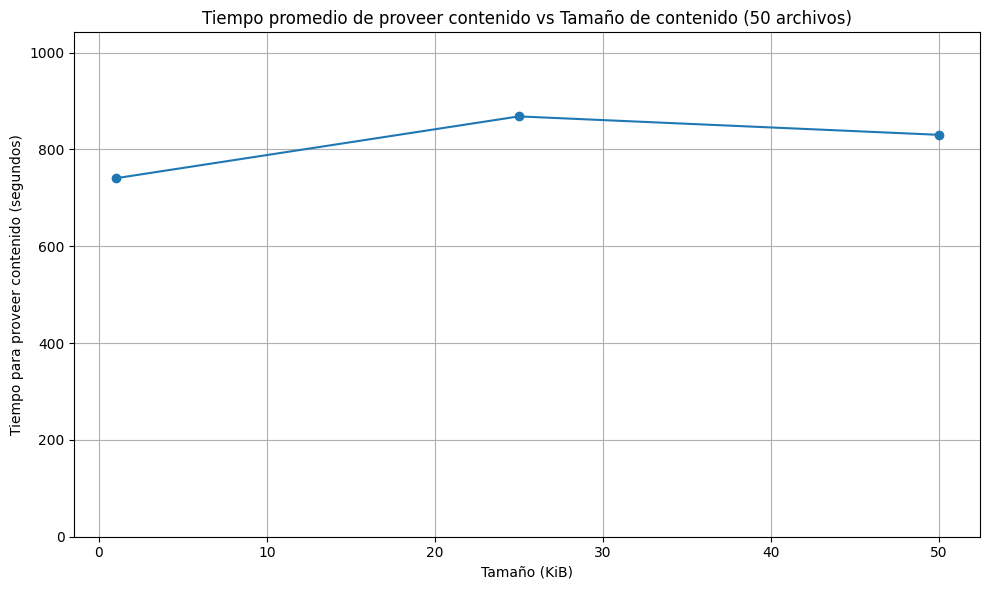
\includegraphics[width=1\linewidth]{img/metricas-ipfs/tiempo-por-tamano.png}
    \caption{Tiempo promedio por tamaño del contenido}
    \label{fig:tiempo-por-tamano.png}
\end{figure}

La cantidad de archivos que tiene el contenido a publicar es la variable que modifica drásticamente el tiempo que tarda un nodo confiable para desplegarlo, como se ve en las figuras. Esto se debe a que la publicación del CID del directorio no es suficiente para que otro nodo pueda obtener el contenido de ese directorio. En cambio, se requiere que se publique todos los archivos y directorios que componen el contenido. Esto también se demuestra con el tiempo constante para publicar el archivo \texttt{service.json}, ya que en todos los casos sigue siendo un sólo archivo. 

\begin{figure}[H]
    \centering
    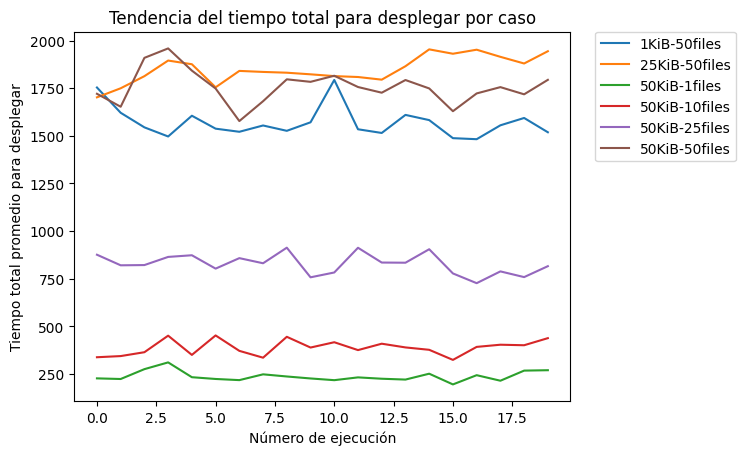
\includegraphics[width=0.9\linewidth]{img/metricas-ipfs/tendencia-desplegar.png}
    \caption{Tendencia del tiempo total promedio para desplegar el contenido en ejecuciones consecutivas.}
    \label{fig:tendencia-desplegar.png}
\end{figure}

Por último, se ve como la tendencia en ejecuciones consecutivas no afecta el tiempo que se tarda en desplegar.

\paragraph{Repositorio de conocimiento}

Las métricas tanto de Astrawiki como Astrachat se ven muy relacionadas, debido a que el grueso del trabajo relacionado a IPFS se realiza con su biblioteca en común, AstraDB. Por ejemplo, el tiempo que tarda un nodo en obtener una nueva versión de un articulo es el similar al que tarda un nodo en recibir un mensaje. Por ello, se prefirió complementar las métricas obtenidas para acentuar el uso específico de AstraDB de cada caso de uso, y evitar métricas repetidas. 

\paragraph{Mensajero en tiempo real}

Las siguientes métricas se obtuvieron con un nodo colaborador y un nodo común. Se levantaron ambos nodos en la misma máquina para poder coordinar ambos nodos y facilitar la obtención de métricas.

Se asume una conexión existente entre el nodo colaborador y el nodo común. Para agilizar la obtención de métricas la conexión directamente mediante las multiaddresses de los nodos, aunque en un caso real se debería encontrar utilizando la DHT. Una vez establecida la conexión el uso es el mismo, por lo que estas métricas no dependen del tipo de mecanismo utilizado para el establecimiento de la conexión.

\subparagraph{Tiempo en enviar un mensaje}

A continuación se muestran los resultados de medir el tiempo que le lleva a un nodo enviar un mensaje a un chat. Para este caso, se asume que el nodo ya está conectado, situación a la que debería llegar un usuario de todos modos antes de enviar un mensaje.

\setlength\tabcolsep{10pt}
\begin{table}[!htbp]
    \centering
    \begin{tabular}{|l|c|c|c|c|c|}
        \hline
        & \textbf{Max} & \textbf{Mean} & \textbf{Min} & \textbf{Std} & \textbf{Median} \\ \hline
        \textbf{short} & 24230 ms & 185.1 ms & 30.25 ms & 765.3 ms & 161.4 ms \\ \hline
        \textbf{medium} & 21870 ms & 175.8 ms & 26.44 ms & 690.1 ms & 153.4 ms \\ \hline
        \textbf{large} & 121000 ms & 265.5 ms & 20.59 ms & 3822 ms & 145.5 ms \\ \hline
    \end{tabular}
    \caption{Tiempo en enviar un mensaje}
\end{table}

Algo a notar son los máximos para cada medición. Estos se deben a una pérdida en la conexión entre nodos que puede ocurrir en el transcurso de una sesión. Sin embargo, son pocos los casos dado el tamaño de la muestra. Por otro lado, el tamaño del mensaje no afecta de forma apreciable el tiempo de envío.

\subparagraph{Tiempo en obtener mensajes}

El gráfico presenta cómo varía el tiempo de respuesta, medido en milisegundos, a medida que crece la cantidad de mensajes en un chat, desde 0 hasta 1000 mensajes en el chat. Se consideran tres tipos de mensajes, y se observa un incremento progresivo en el tiempo necesario para obtenerlos. Esta métrica se obtuvo midiendo el tiempo requerido para recuperar todos los mensajes en chats con diferentes tamaño de contenido. Además, se eliminaron los \textit{outliers} por pérdida de conexión para poder visualizar mejor la tendencia en general.

\begin{figure}[h!]
    \centering
    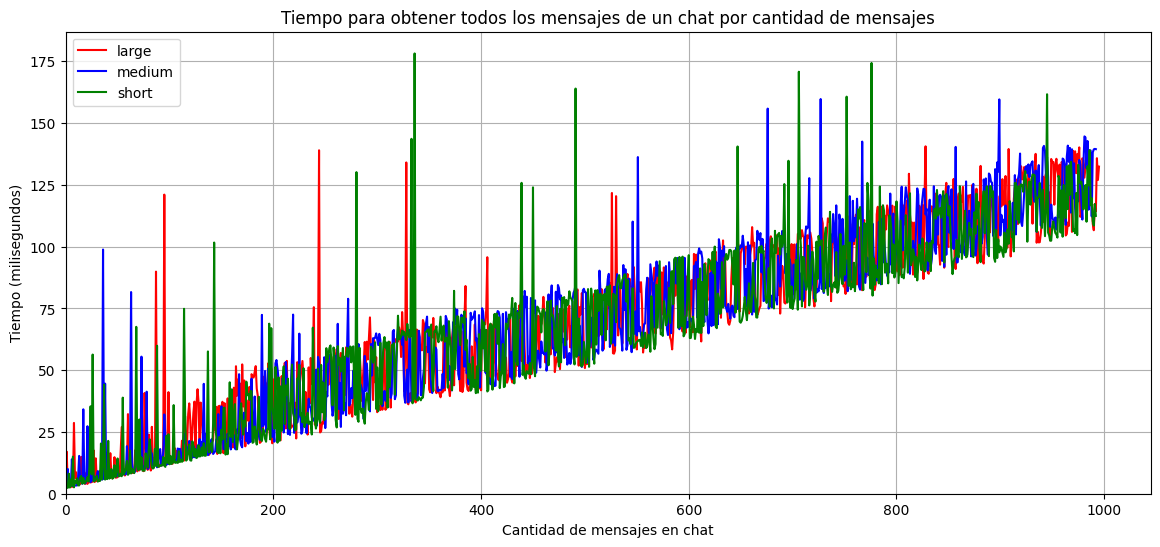
\includegraphics[width=1\linewidth]{img/metricas-ipfs/tiempo-para-obtener-por-cant-msjs.png}
    \caption{Tiempo para obtener mensajes de un chat según el tamaño del chat}
    \label{fig:ipfs-get-message-graphic.png}
\end{figure}

\setlength\tabcolsep{10pt}
\begin{table}[!htbp]
    \centering
    \begin{tabular}{|l|c|c|c|c|c|}
        \hline
        & \textbf{Max} & \textbf{Mean} & \textbf{Min} & \textbf{Std} & \textbf{Median} \\ \hline
        \textbf{short} & 5665 ms & 79.45 ms & 2.340 ms & 248.8 ms & 69.19 ms \\ \hline
        \textbf{medium} & 8471 ms & 85.47 ms & 2.718 ms & 359.4 ms & 70.14 ms \\ \hline
        \textbf{large} & 3905 ms & 76.96 ms & 2.642 ms & 161.2 ms & 69.15 ms \\ \hline
    \end{tabular}
    \caption{Tiempo en obtener mensajes}
\end{table}  

\subparagraph{Tiempo entre enviar y recibir un mensaje}

Esta métrica calcula el tiempo que tarda el nodo común en recibir un mensaje enviado por el nodo colaborador. Para ello se utiliza el \texttt{EventEmitter} integrado en Astrachat, logrando una medición exacta del trayecto de un mensaje para una conexión ya establecida. Al igual que en los demás casos, existen outliers provenientes de pérdidas de conexión, los cuáles se pueden observar en los máximos obtenidos. Sin embargo, la desviación estándar y el valor promedio y mediano indican que estos no son frecuentes.

\setlength\tabcolsep{10pt}
\begin{table}[!htbp]
    \centering
    \begin{tabular}{|l|c|c|c|c|c|}
        \hline
        & \textbf{Max} & \textbf{Mean} & \textbf{Min} & \textbf{Std} & \textbf{Median} \\ \hline
        \textbf{short} & 22790 ms & 298.1 ms & 47.85 ms & 1341 ms & 198.8 ms \\ \hline
        \textbf{medium} & 18050 ms & 227.0 ms & 40.89 ms & 800.4 ms & 195.0 ms \\ \hline
        \textbf{large} & 20680 ms & 285.8 ms & 64.47 ms & 1264 ms & 196.1 ms \\ \hline
    \end{tabular}
    \caption{Tiempo entre enviar y recibir un mensaje}
\end{table}  
\subsection{Blockchain}

\subsubsection{Costos}

\paragraph{Swarm}
Al deployar el sitio web es necesario contar con \textit{postage stamps} que son la manera de pagar por el uso del almacenamiento en Swarm. Cada actualización que se realice al sitio requiere de \textit{postage stamps} y, además, estos tienen fecha de vencimiento por lo que es necesario volver a pagar frecuentemente. Hay que tener en cuenta que dichos \textit{postage stamps} se pagan en la criptomoneda BZZ que fluctúa de valor con respecto al dólar estadounidense. La obtención del sitio web no requiere de costo alguno, por lo que desde el punto de vista de un usuario lector de la aplicación no sería necesario pagar.

<TODO: medir cuánto es el costo aproximado en USD o BZZ>

\paragraph{Ethereum}
Se utiliza la moneda ETH para pagar por cada transacción, esto incluye tanto el despliegue de cada \textit{smart contract} como también cada modificación al estado de los mismos. Por lo tanto, el usuario final de la aplicación termina pagando por la creación y edición de cada artículo en el repositorio de conocimiento, y por cada mensaje enviado en el mensajero en tiempo real. Por otro lado, para las operaciones de lectura no se tiene que pagar nada. A este monto que tiene que pagar el usuario se lo llama gas y varía con respecto a las operaciones que realiza el método que se ejecuta al llamar a un \textit{smart contract} y, también, con respecto a la congestión de la red, es decir a mayor congestión mayor será el costo.

\begin{figure}[H]
    \centering
    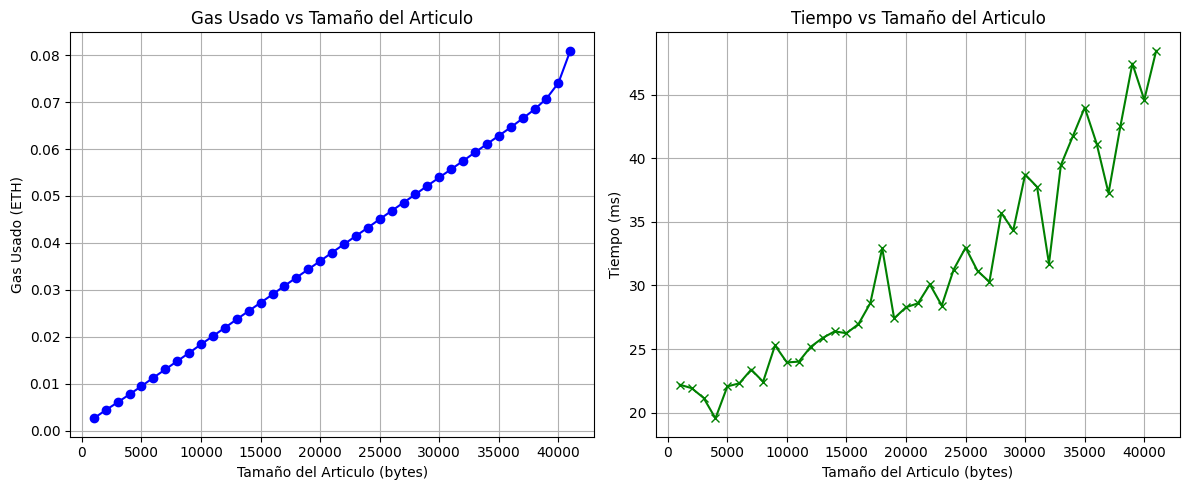
\includegraphics[width=1\linewidth]{img/aw-eth-bytes-articulo-incremental.png}
    \caption{Tiempo y gas usado al crear artículos con tamaño de bytes creciente}
    \label{fig:aw-eth-bytes-articulo-incremental.png}
\end{figure}

\subsubsection{Experiencia de desarrollo} % Developer Experience

\paragraph{Swarm}
En Swarm existe la herramienta de terminal swarm-cli \cite{swarm-cli} con la cual se puede interactuar con un nodo de Swarm. También el equipo de Swarm provee una Github Action que permite la posibilidad de automatizar el despliegue generando un pipeline que utilice dicha herramienta.

En cuanto a un ambiente de pruebas o \textit{staging}, si bien no existe un \textit{gateway} público que interactúe con la \textit{testnet}, es posible levantar uno propio que sí lo haga apuntando a la \textit{testnet} de Sepolia usando la herramienta gateway-proxy \cite{gateway-proxy}.

\paragraph{Ethereum}
Con la librería web3.js se puede interactuar con un nodo de Ethereum y realizar un despliegue de la aplicación. Además, con las herramientas de Hardhat se puede levantar una red de prueba que facilita el desarrollo local.

\subsubsection{Viabilidad}

\paragraph{Swarm}
Resulta más conveniente para sitios web o recursos estáticos, al igual que IPFS. Por otro lado, al ser una tecnología de almacenamiento no es posible la ejecución de código.

A diferencia de IPFS, Swarm cuenta con incentivos incluidos (por medio de la moneda BZZ), esto significa que para deployar contenido en la red es necesario pagar. Al hacerlo te asegura que el mismo va a estar disponible durante el tiempo equivalente al costo pagado, es decir, que no es necesario pinear los archivos puesto que se encuentran en la red con un TTL.

\paragraph{Ethereum}
Su punto fuerte es la ejecución de código, por lo cual es útil para funcionar como backend de aplicaciones web. Como hemos visto, por el costo de almacenamiento de los smart contracts, no es recomendable para recursos como imágenes, videos o incluso strings de texto muy largos como lo realizado en el repositorio de conocimiento. 

Los eventos pueden resultar útil para la interacción en tiempo real requerida en el mensajero, pero lo positivo de esto queda opacado por el hecho de necesitar pagar por cada interacción, en el caso del mensajero por cada mensaje enviado. Esto se puede volver costoso rápidamente, además de tedioso al momento de utilizar la aplicación. Se pueden explorar alternativas para reducir esta fricción, como por ejemplo, que el contrato tenga un balance de tokens para ser gastados, lo cual haría que el usuario no tenga que confirmar cada transacción de mensaje enviado si no que directamente el contrato lo extrae de su balance; entre otras posibilidades.

\subsubsection{Performance\label{performance-blockchain}}

\paragraph{Astrachat}

Las siguientes métricas se obtuvieron levantando una instancia local de Hardhat \cite{hardhat} y ejecutando 850 muestras, 3 veces cada una y con 3 mensajes de largo distinto:

\begin{itemize}
    \item \textit{short}: mensaje de 1 palabra. ''\textit{Lorem}''
    \item \textit{medium}: mensaje de 10 palabras. ''\textit{Lorem ipsum dolor sit amet, consectetur adipiscing elit. Aliquam elementum.}''
    \item \textit{large}: mensaje de 30 palabras. ''\textit{Lorem ipsum dolor sit amet, consectetur adipiscing elit. Aliquam ex risus, porttitor sed lacus id, egestas lobortis purus. Curabitur consectetur metus ut est vehicula egestas. Class aptent taciti sociosqu ad.}''
\end{itemize}

El tamaño de las palabras elegidas representa el largo de los mensajes más comunes que suelen enviarse en un chat.

Hay que tener en cuenta que los tiempos obtenidos corresponden al que le toma a la transacción ejecutarse en una máquina local. En un caso real, existe un tiempo mayor de red y de interacción del usuario con la \textit{wallet} para confirmar la transacción.

A partir de los datos obtenidos se calcularon el máximo (\textbf{Max}), mínimo (\textbf{Min}), la media (\textbf{Mean}), el desvío estándar (\textbf{Std}) y la mediana (\textbf{Median}).

\subparagraph{Tiempo en enviar un mensaje}

La primer métrica tomada corresponde al tiempo que tarda en enviarse un mensaje.

\setlength\tabcolsep{10pt}
\begin{table}[!htbp]
    \centering
    % \begin{tabular}{|m{5em}|m{5em}|}
    \begin{tabular}{|*4{c|}}
    \hline
    & \textbf{short} & \textbf{medium} & \textbf{large} \\
    \hline
    \textbf{Max} & 10.93 ms & 10.34 ms & 10.68 ms \\
    \hline
    \textbf{Mean} & 6.12 ms & 6.26 ms & 6.44 ms \\
    \hline
    \textbf{Min} & 5.09 ms & 5.24 ms & 5.36 ms \\
    \hline
    \textbf{Std} & 0.74 ms & 0.60 ms & 0.70 ms \\
    \hline
    \textbf{Median} & 6.01 ms & 6.20 ms & 6.37 ms\\
    \hline
    \end{tabular}
    \caption{Tiempo en enviar un mensaje}
\end{table}

Se puede observar que los tiempos entre los tamaños de mensajes no varían demasiado.

\subparagraph{Gas usado para enviar un mensaje}

La siguiente tabla muestra el valor (en ETH y USD) de enviar el mismo mensaje corto. El precio tomado para la conversión de ETH a dólar es el de la fecha del 5 de junio de 2025 a las 19:00hs de \$2439.17 de la página \href{https://coinmarketcap.com/currencies/ethereum/}{Coinmarketcap}.

\setlength\tabcolsep{10pt}
\begin{table}[H]
    \centering
    \begin{tabular}{|c|cc|cc|cc|}
    \hline
     & \multicolumn{2}{c|}{\textbf{short}} & \multicolumn{2}{c|}{\textbf{medium}} & \multicolumn{2}{c|}{\textbf{large}} \\ \hline
     & \multicolumn{1}{c|}{\textbf{ETH}} & \multicolumn{1}{c|}{\textbf{USD}} & \multicolumn{1}{c|}{\textbf{ETH}} & \multicolumn{1}{c|}{\textbf{USD}} & \multicolumn{1}{c|}{\textbf{ETH}} & \multicolumn{1}{c|}{\textbf{USD}} \\
     \hline
    \textbf{Max} & \multicolumn{1}{l|}{0.00042043} & 1.03 & \multicolumn{1}{l|}{0.00060668} & 1.48 & \multicolumn{1}{l|}{0.00085774} & 2.09 \\
    \hline
    \textbf{Mean} & \multicolumn{1}{l|}{0.00034257} & 0.84 & \multicolumn{1}{l|}{0.00051325} & 1.25 & \multicolumn{1}{l|}{0.00074335} & 1.81 \\
    \hline
    \textbf{Min} & \multicolumn{1}{l|}{0.00034221} & 0.83 & \multicolumn{1}{l|}{0.00051274} & 1.25 & \multicolumn{1}{l|}{0.00074264} & 1.81 \\
    \hline
    \textbf{Std} & \multicolumn{1}{l|}{0.00000331} & 0.01 & \multicolumn{1}{l|}{0.00000434} & 0.01 & \multicolumn{1}{l|}{0.00000579} & 0.01 \\
    \hline
    \textbf{Median} & \multicolumn{1}{l|}{0.00034221} & 0.83 & \multicolumn{1}{l|}{0.00051274} & 1.25 & \multicolumn{1}{l|}{0.00074264} & 1.81 \\
    \hline
    \end{tabular}
    \caption{Precio y gas usado para enviar un mensaje}
\end{table}

Según los resultados obtenidos se puede decir que para enviar un mensaje cuesta más de 1 dólar.

\subparagraph{Tiempo en obtener mensajes}

Para esta métrica se tomó el tiempo en obtener todos los mensajes para un chat el cual iba teniendo cada vez más mensajes (desde 0 hasta 850 mensajes). El gráfico muestra para los 3 tipos de mensajes, cómo el tiempo (en milisegundos) se va incrementando a medida que hay más mensajes en el chat.

\begin{figure}[h!]
    \centering
    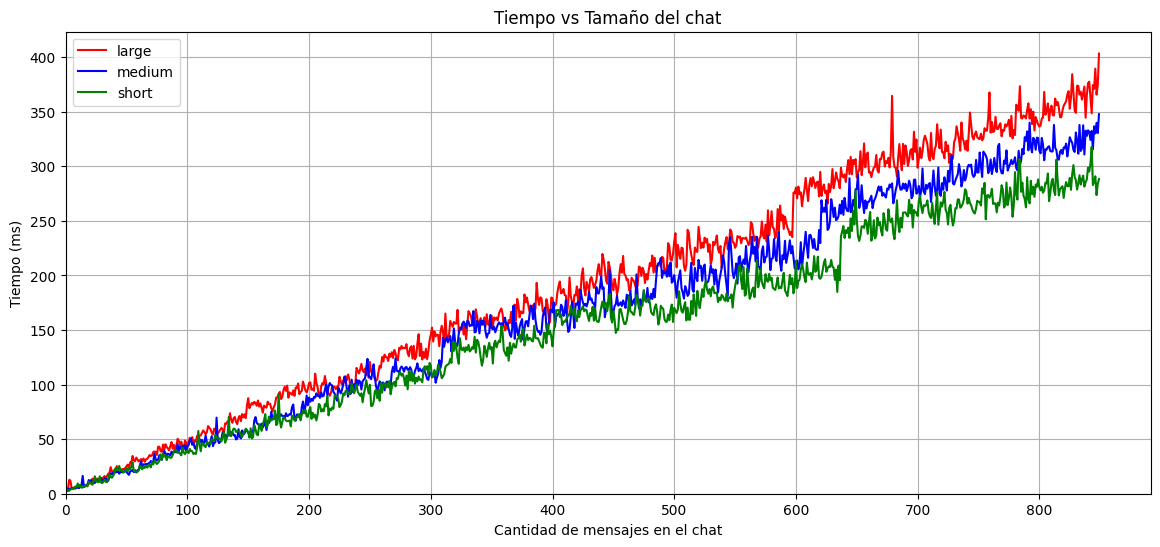
\includegraphics[width=1\linewidth]{img/blockchain-get-message-graphic.png}
    \caption{Tiempo para obtener mensajes de un chat según el tamaño del chat}
    \label{fig:blockchain-get-message-graphic.png}
\end{figure}

\subparagraph{Tiempo entre enviar y recibir un mensaje (mismo usuario)}

En esta métrica se midió el tiempo que tarda en un mensaje desde que es enviado a ser recibido por el canal de escucha de nuevos mensajes para un mismo usuario.

\setlength\tabcolsep{10pt}
\begin{table}[H]
    \centering
    \begin{tabular}{|*4{c|}}
    \hline
     & \textbf{short} & \textbf{medium} & \textbf{large} \\
    \hline
    \textbf{Max} & 38.12 ms & 28.97 ms & 24.66 ms \\
    \hline
    \textbf{Mean} & 5.42 ms & 5.76 ms & 5.76 ms \\
    \hline
    \textbf{Min} & 4.26 ms & 4.31 ms & 4.46 ms \\
    \hline
    \textbf{Std} & 1.62 ms & 1.74 ms & 0.94 ms \\
    \hline
    \textbf{Median} & 4.66 ms & 5.05 ms & 5.6 ms \\
    \hline
    \end{tabular}
    \caption{Tiempo en enviar y recibir un mensaje (mismo usuario)}
    \label{tab:tiempo-send-recv-same-user}
\end{table}

\subparagraph{Tiempo entre enviar y recibir un mensaje (distintos usuarios)}

Esta métrica calcula el tiempo que tarda un segundo usuario en recibir un mensaje enviado por un primer usuario.

\setlength\tabcolsep{10pt}
\begin{table}[H]
    \centering
    \begin{tabular}{|*4{c|}}
    \hline
     & \textbf{short} & \textbf{medium} & \textbf{large} \\
    \hline
    \textbf{Max} & 13.19 ms & 10.92 ms & 13.95 ms \\
    \hline
    \textbf{Mean} & 5.61 ms & 5.84 ms & 5.96 ms \\
    \hline
    \textbf{Min} & 4.59 ms & 4.53 ms & 4.65 ms \\
    \hline
    \textbf{Std} & 0.97 ms & 1.28 ms & 0.72 ms \\
    \hline
    \textbf{Median} & 5.53 ms & 5.06 ms & 5.89 ms \\
    \hline
    \end{tabular}
    \caption{Tiempo en enviar y recibir un mensaje (distintos usuarios)}
    \label{tab:tiempo-send-recv-diff-user}
\end{table}

Si comparamos las tablas de tiempos de enviar y recibir un mensaje (\ref{tab:tiempo-send-recv-same-user} y \ref{tab:tiempo-send-recv-diff-user}) vemos que los tiempos son parecidos. Si bien los máximos de la primer tabla son mayores que los de la segunda y los datos están más dispersos, para los demás valores de la segunda tabla estos tienden a ser ligeramente mayores. En este caso particular, si se hiciera una prueba entre 2 usuarios de distintas partes del mundo el tiempo de conexión seguramente pesaría más.

\subsection{Resumen}

Resumiendo, y a modo de comparación entre ecosistemas, podemos concluir con lo siguiente:

\setlength\tabcolsep{1pt}
\begin{table}[H]
    \centering
    \begin{tabular}{|m{7em}|m{14em}|m{14em}|}
    \hline
     & \textbf{IPFS} & \textbf{Blockchain} \\
    \hline
    \textbf{Costos} & Bajos o nulos & Escala con el uso de la aplicación \\
    \hline
    \textbf{Desarrollo} &  & Existen herramientas que facilitan el desarrollo y el despliegue \\
    \hline
    \textbf{Viabilidad} & & Sitios estáticos y aplicaciones CRUD \\
    \hline
    \textbf{Performance} & & \\
    \hline
    \end{tabular}
    \caption{Comparación entre los ecosistemas de IPFS y Blockchain}
\end{table}